\begin{apendicesenv}

\partapendices

\chapter{Análise dos Percentis do Estudo de Caso} \label{anex:percentis}

Neste anexo contém os gráficos relacionados com a análise de percentis de cada
uma das métricas de vulnerabilidades apresentadas em \ref{cap:metricas_vuln}
do
projeto \emph{Linux Kernel}, sendo esses parte dos resultados descritos na seção
\ref{subsec:teste_hipotese}.


\begin{figure}[h]
  \centering
  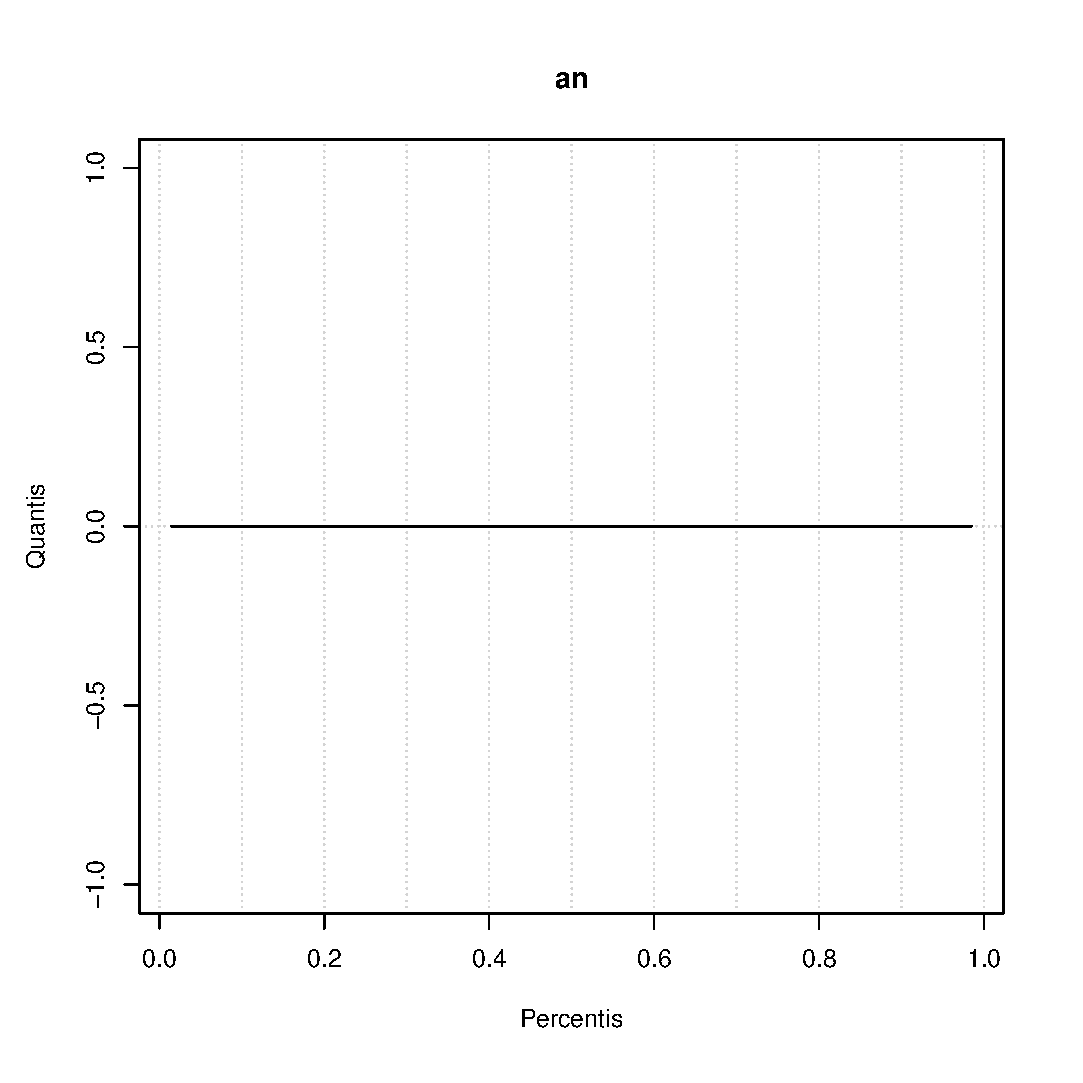
\includegraphics[width=0.7\textwidth]
      {dados/linux/an.eps}
  \caption{Gráfico de Percentis da métrica AN}
\end{figure}

\newpage

\begin{figure}[h]
  \centering
  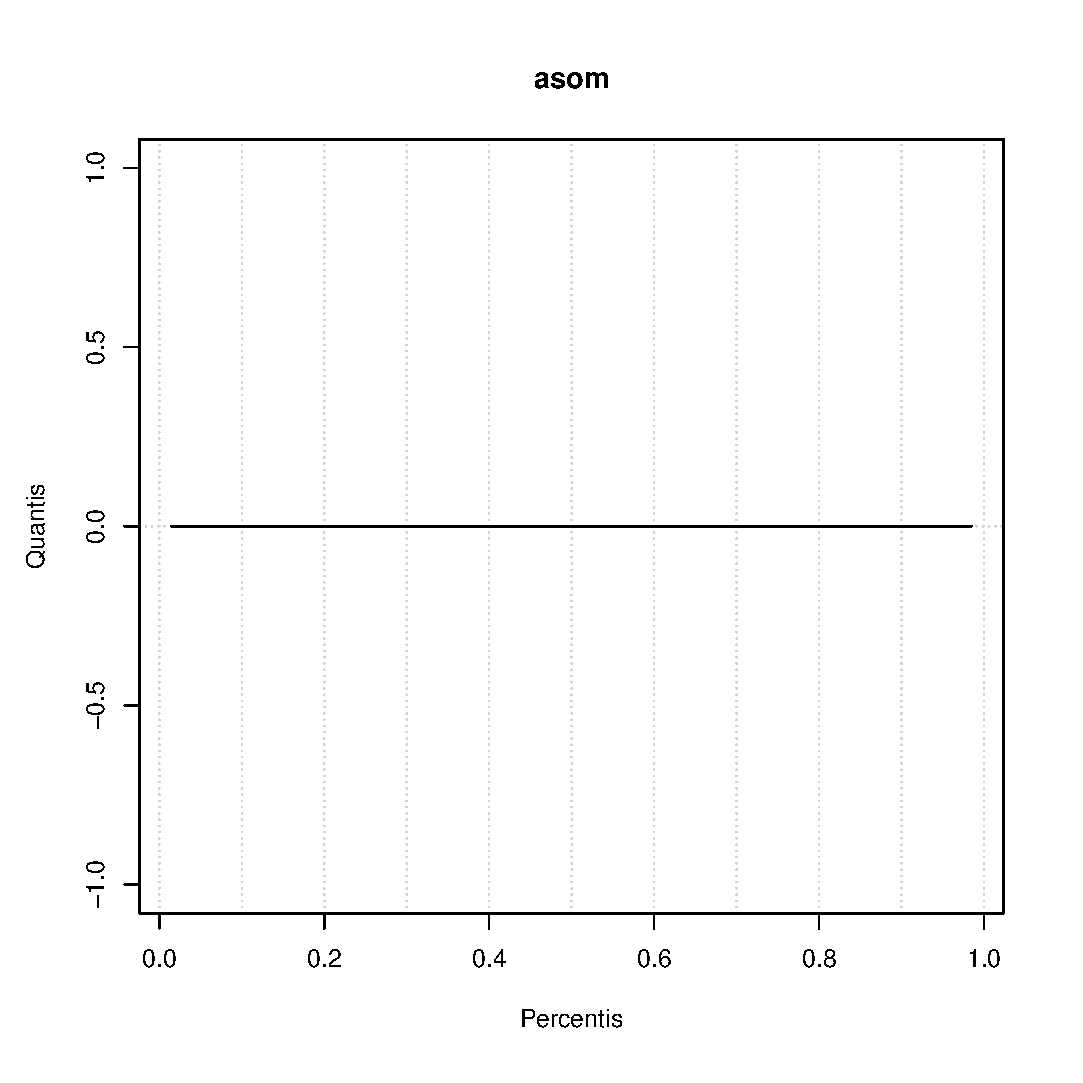
\includegraphics[width=0.6\textwidth]
      {dados/linux/asom.eps}
  \caption{Gráfico de Percentis da métrica ASOM}
  \label{graphic:asom}
\end{figure}

\begin{figure}[h]
  \centering
  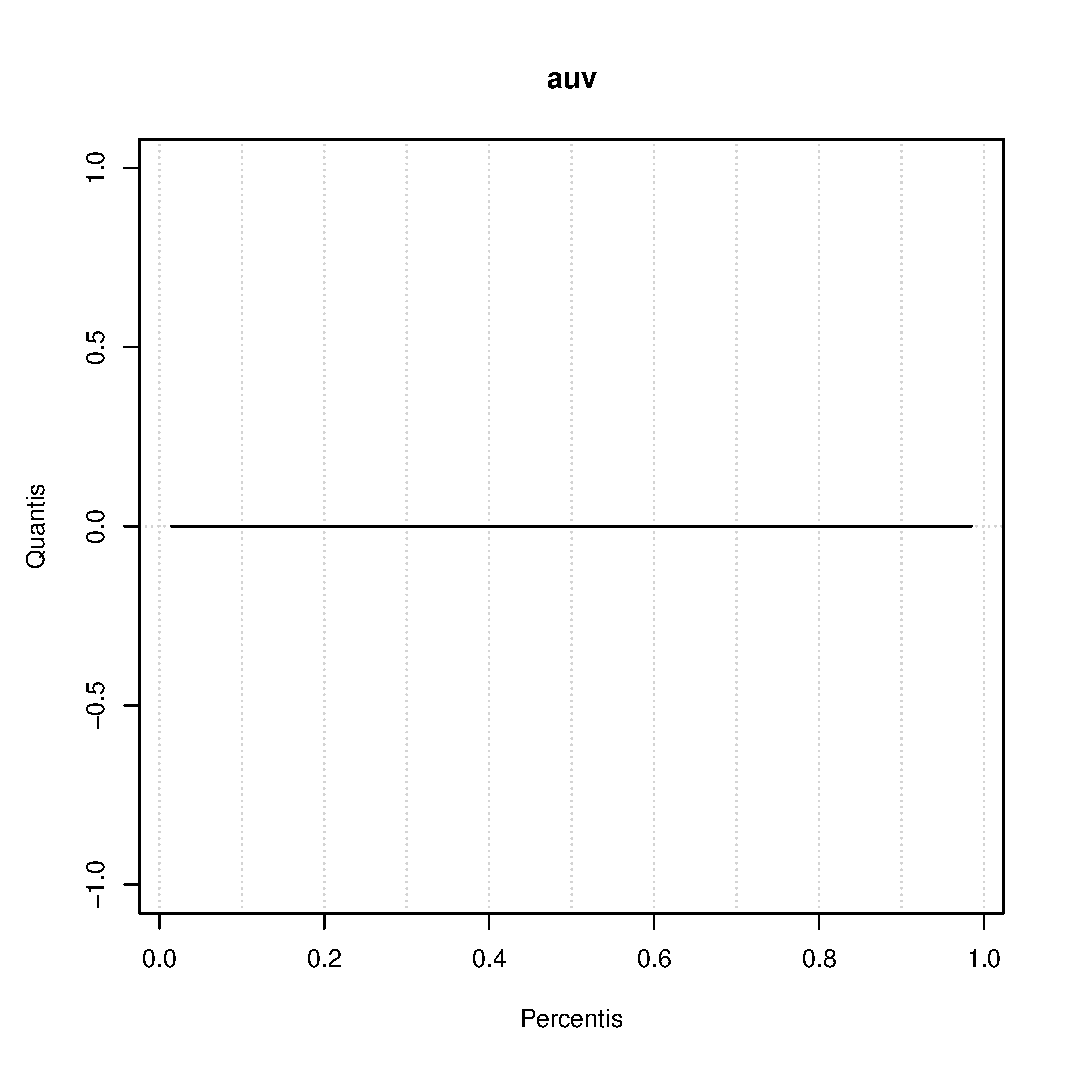
\includegraphics[width=0.6\textwidth]
      {dados/linux/auv.eps}
  \caption{Gráfico de Percentis da métrica AUV}
\end{figure}

\newpage

\begin{figure}[h]
  \centering
  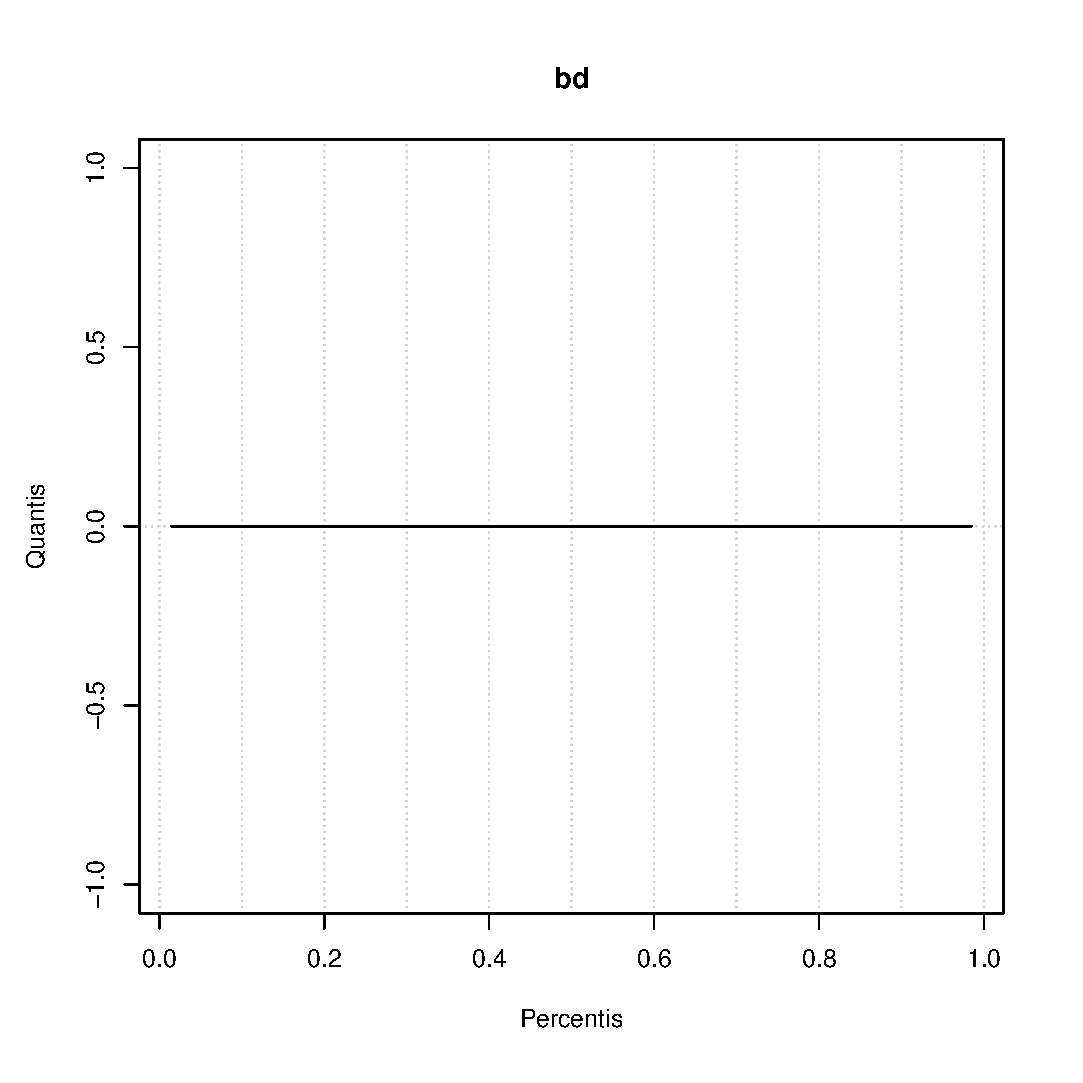
\includegraphics[width=0.6\textwidth]
      {dados/linux/bd.eps}
  \caption{Gráfico de Percentis da métrica BD}
\end{figure}

\begin{figure}[h]
  \centering
  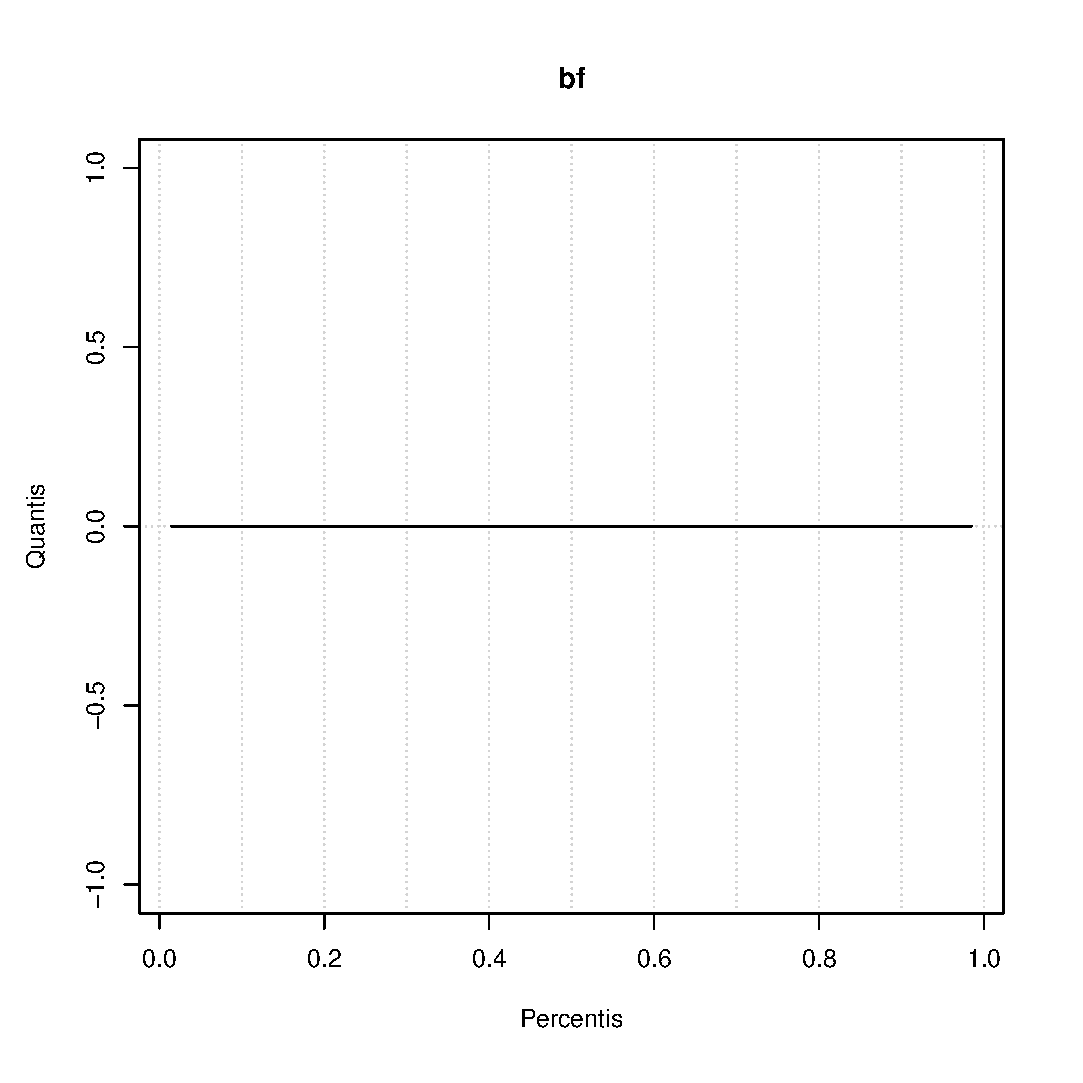
\includegraphics[width=0.6\textwidth]
      {dados/linux/bf.eps}
  \caption{Gráfico de Percentis da métrica BF}
\end{figure}

\newpage

\begin{figure}[h]
  \centering
  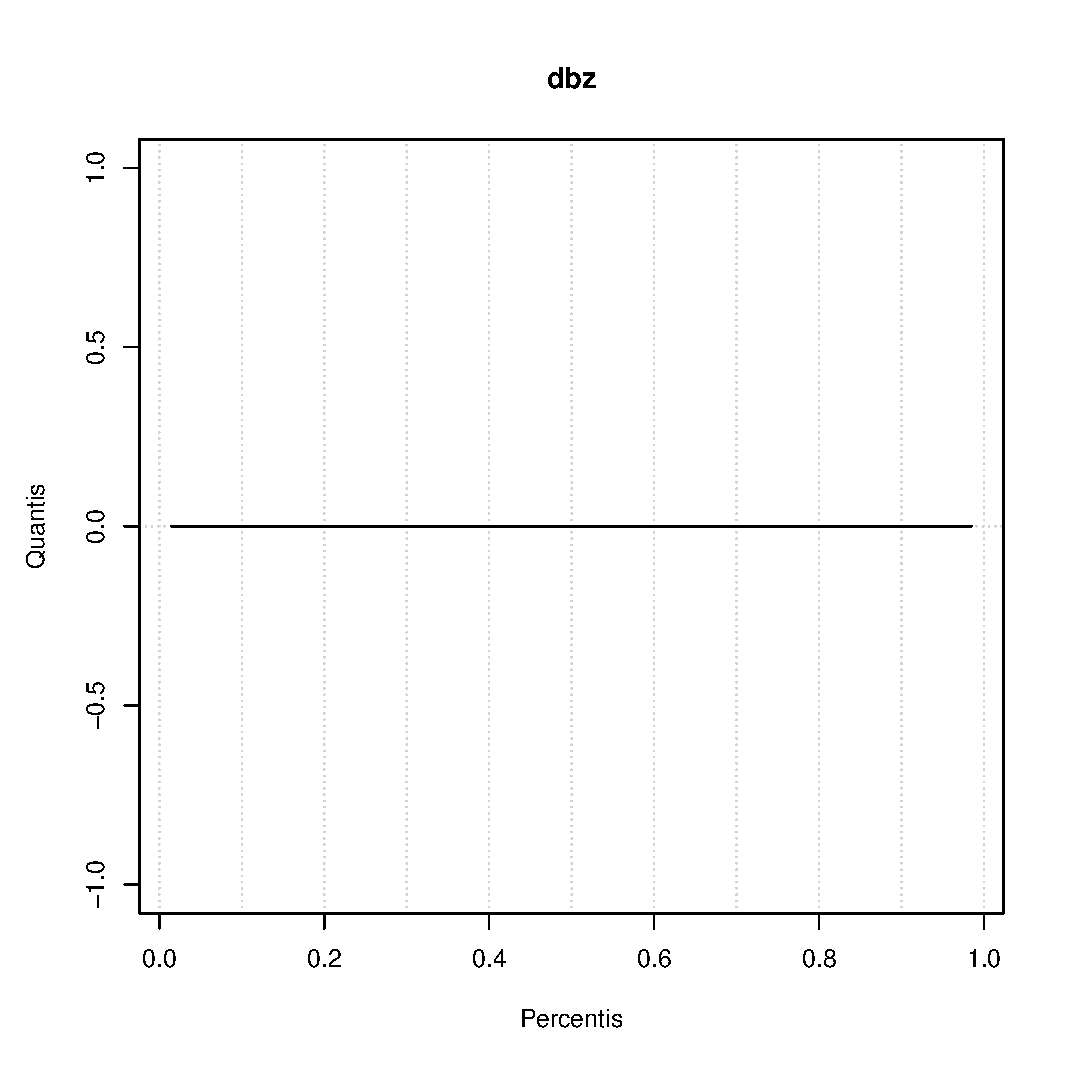
\includegraphics[width=0.6\textwidth]
      {dados/linux/dbz.eps}
  \caption{Gráfico de Percentis da métrica DBZ}
\end{figure}

\begin{figure}[h]
  \centering
  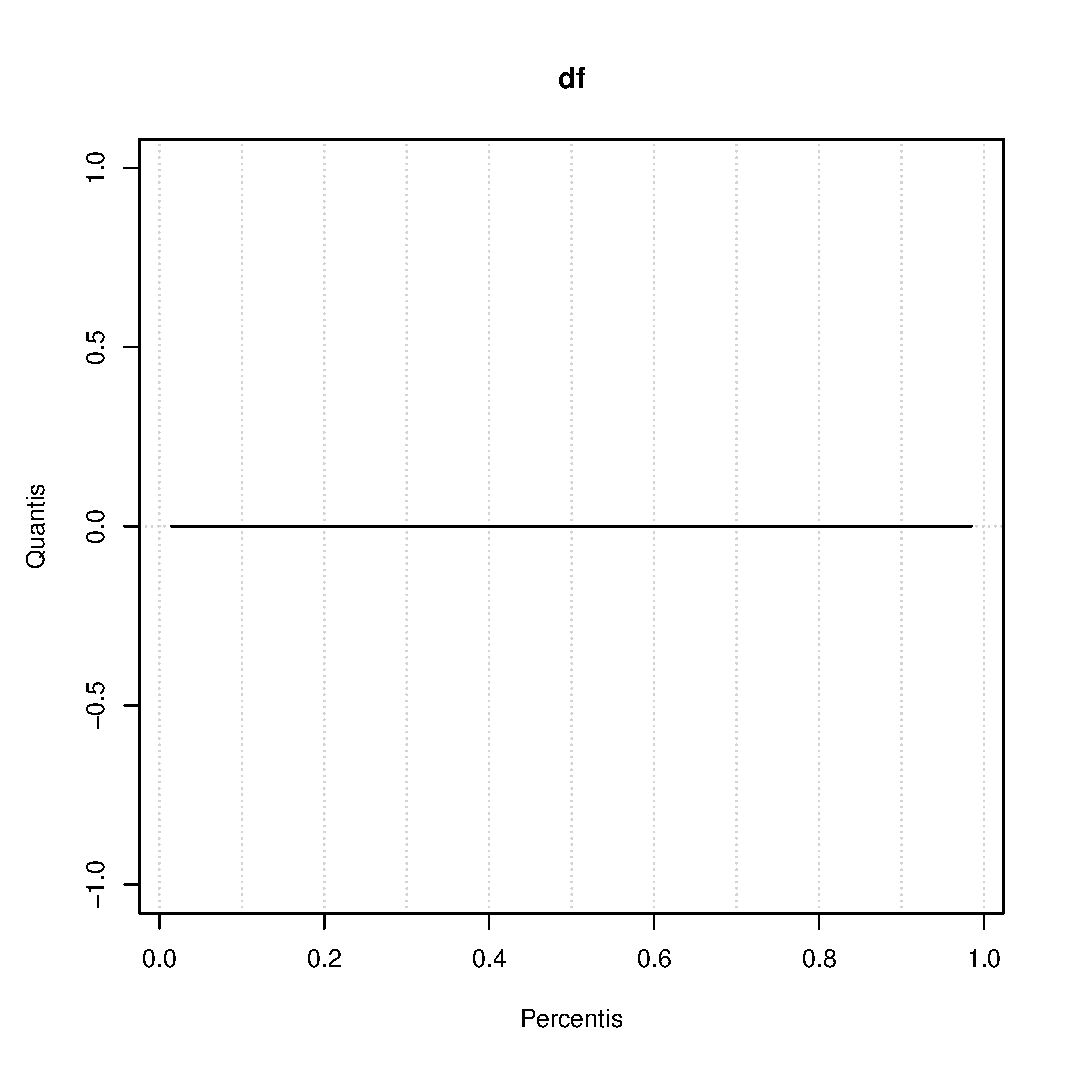
\includegraphics[width=0.6\textwidth]
      {dados/linux/df.eps}
  \caption{Gráfico de Percentis da métrica DF}
\end{figure}

\newpage

\begin{figure}[h]
  \centering
  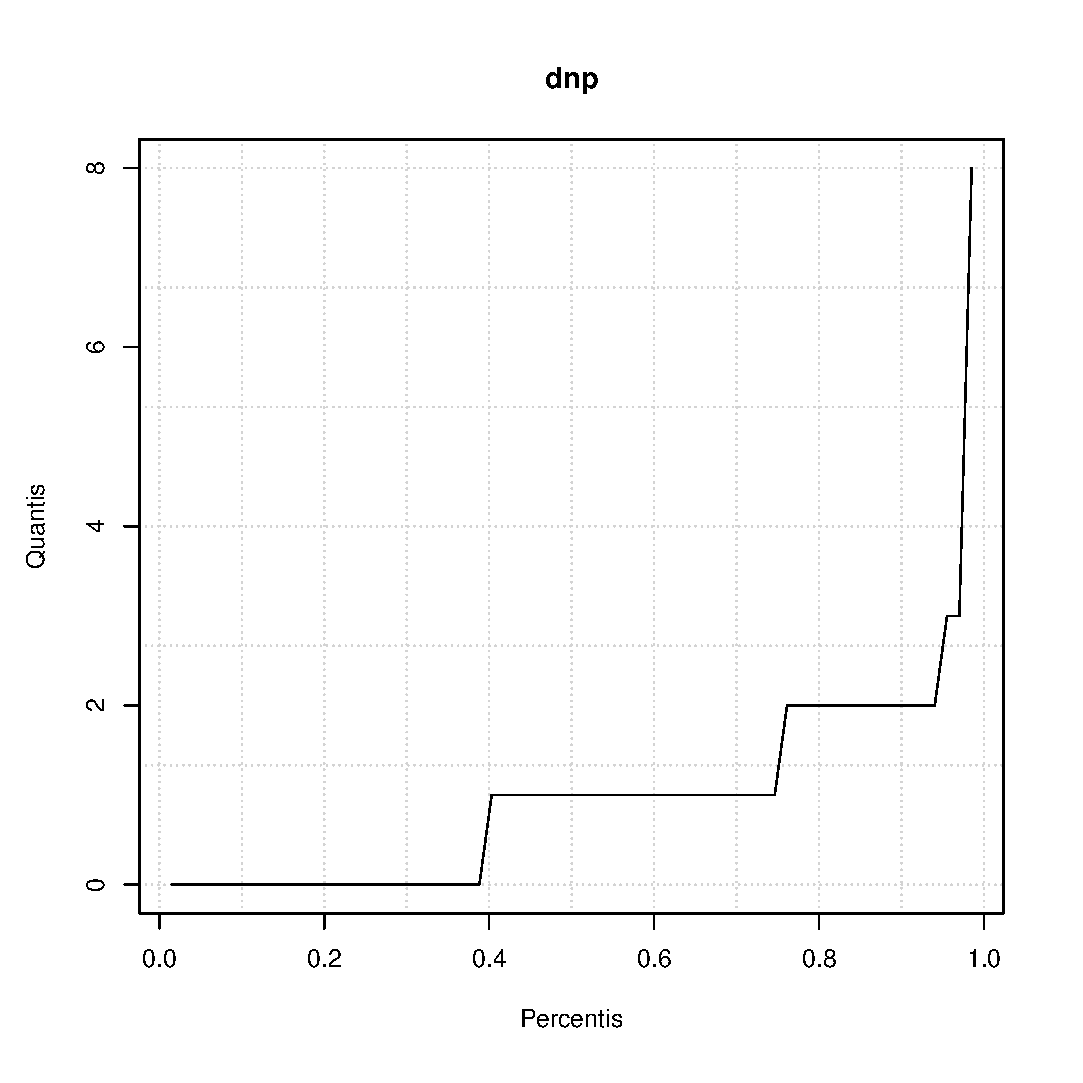
\includegraphics[width=0.6\textwidth]
      {dados/linux/dnp.eps}
  \caption{Gráfico de Percentis da métrica DNP}
  \label{graphic:dnp}
\end{figure}

\begin{figure}[h]
  \centering
  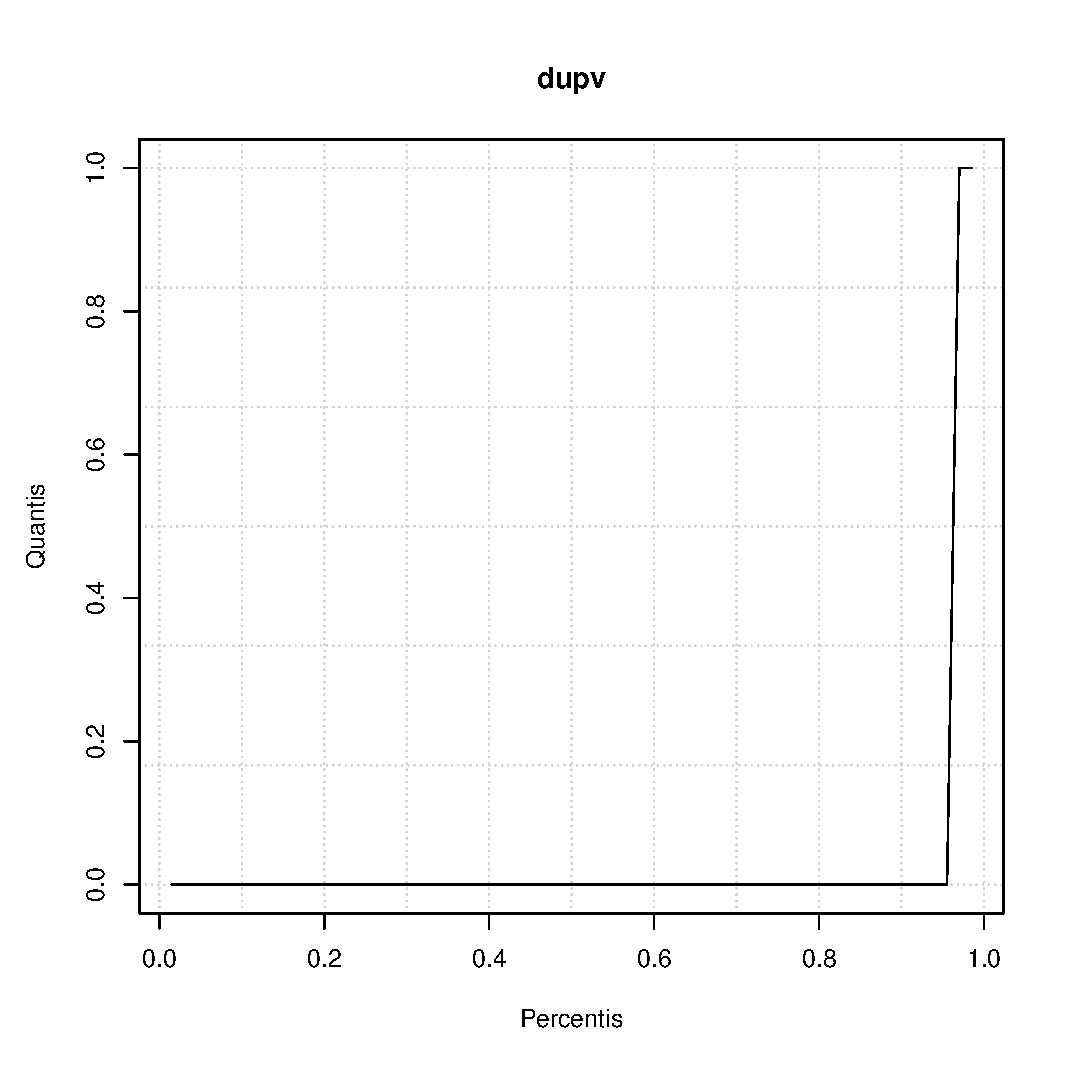
\includegraphics[width=0.6\textwidth]
      {dados/linux/dupv.eps}
  \caption{Gráfico de Percentis da métrica DUPV}
  \label{graphic:dupv}
\end{figure}

\newpage

\begin{figure}[h]
  \centering
  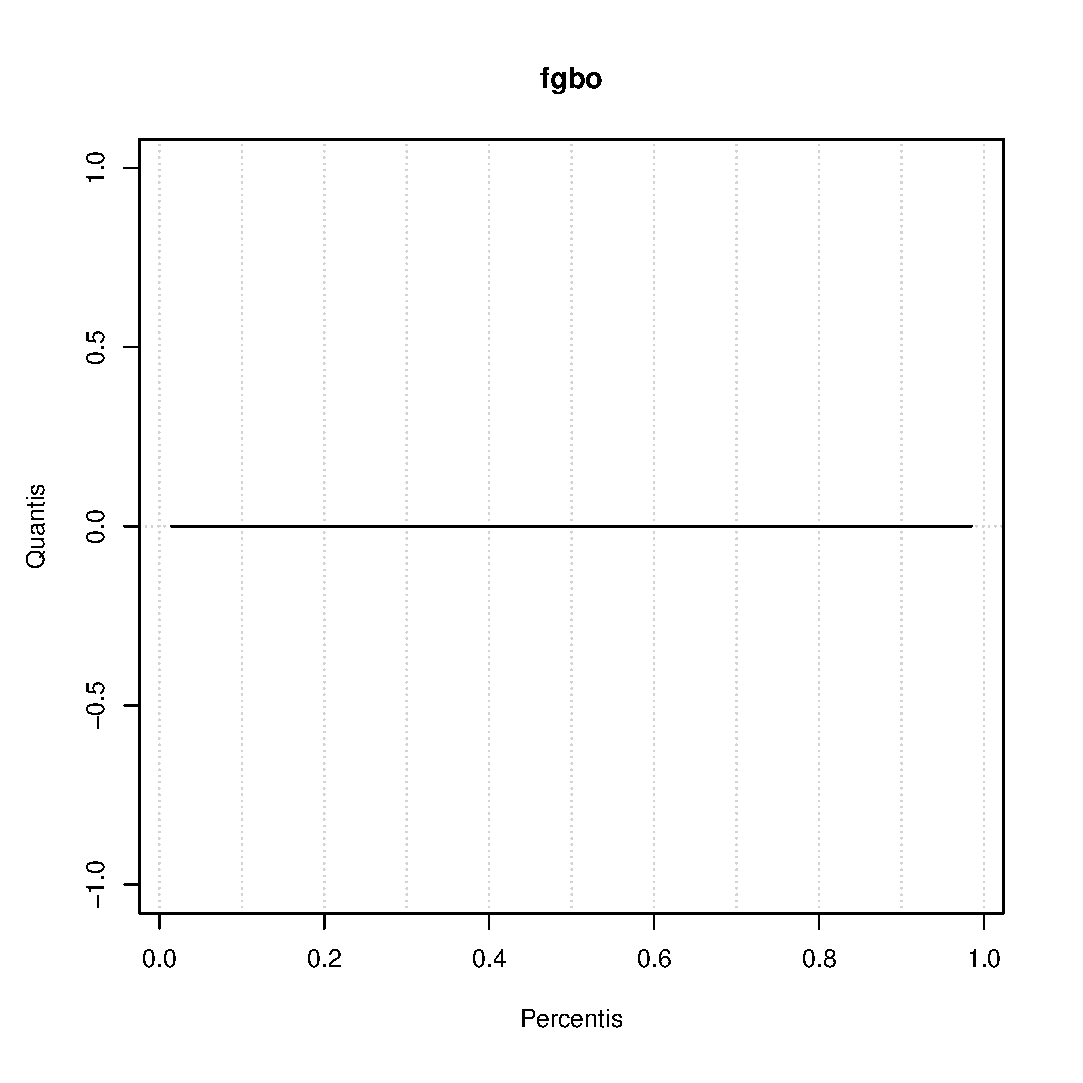
\includegraphics[width=0.6\textwidth]
      {dados/linux/fgbo.eps}
  \caption{Gráfico de Percentis da métrica FGBO}
\end{figure}

\begin{figure}[h]
  \centering
  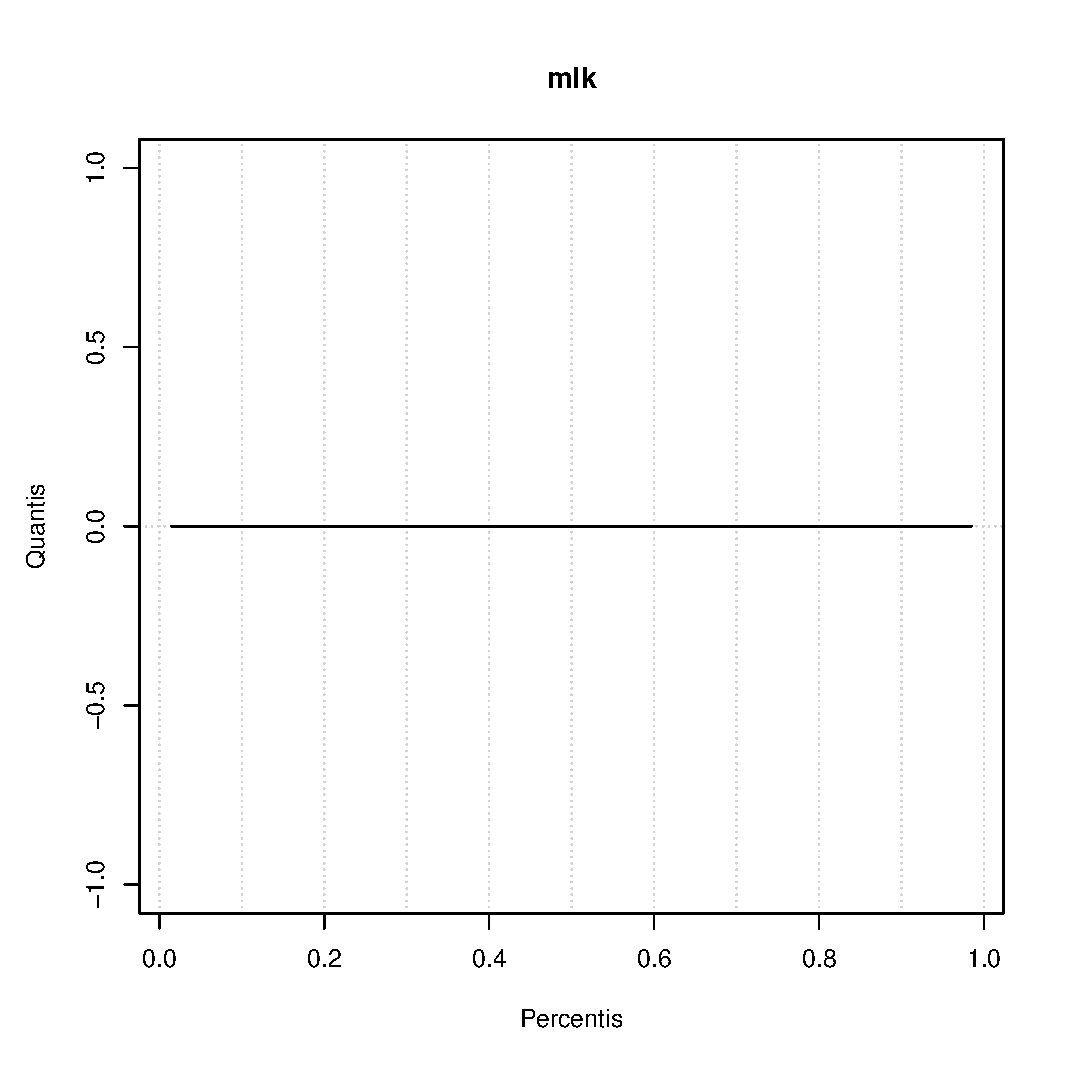
\includegraphics[width=0.6\textwidth]
      {dados/linux/mlk.eps}
  \caption{Gráfico de Percentis da métrica MLK}
\end{figure}

\newpage

\begin{figure}[h]
  \centering
  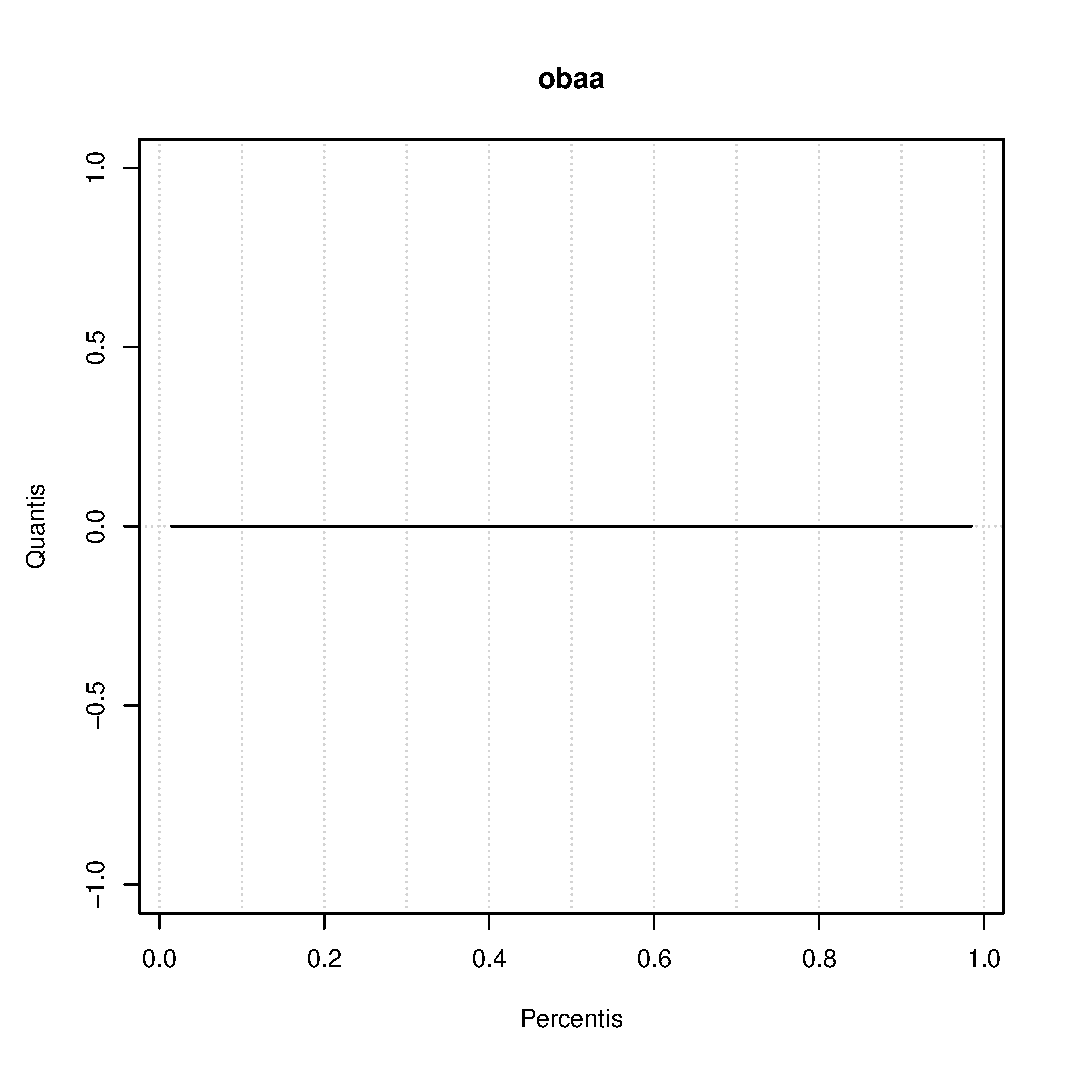
\includegraphics[width=0.6\textwidth]
      {dados/linux/obaa.eps}
  \caption{Gráfico de Percentis da métrica OBAA}
\end{figure}

\begin{figure}[h]
  \centering
  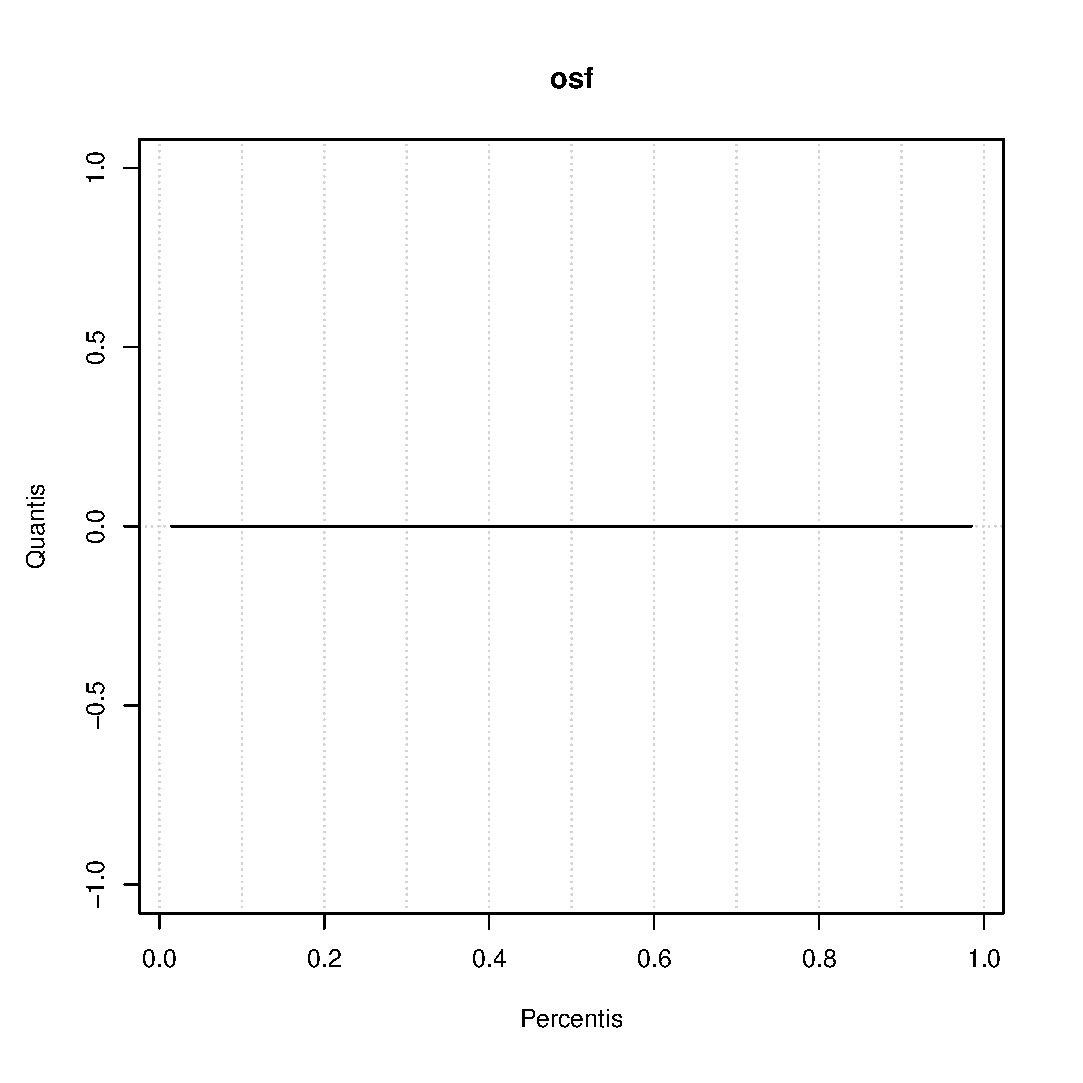
\includegraphics[width=0.6\textwidth]
      {dados/linux/osf.eps}
  \caption{Gráfico de Percentis da métrica OSF}
\end{figure}

\newpage

\begin{figure}[h]
  \centering
  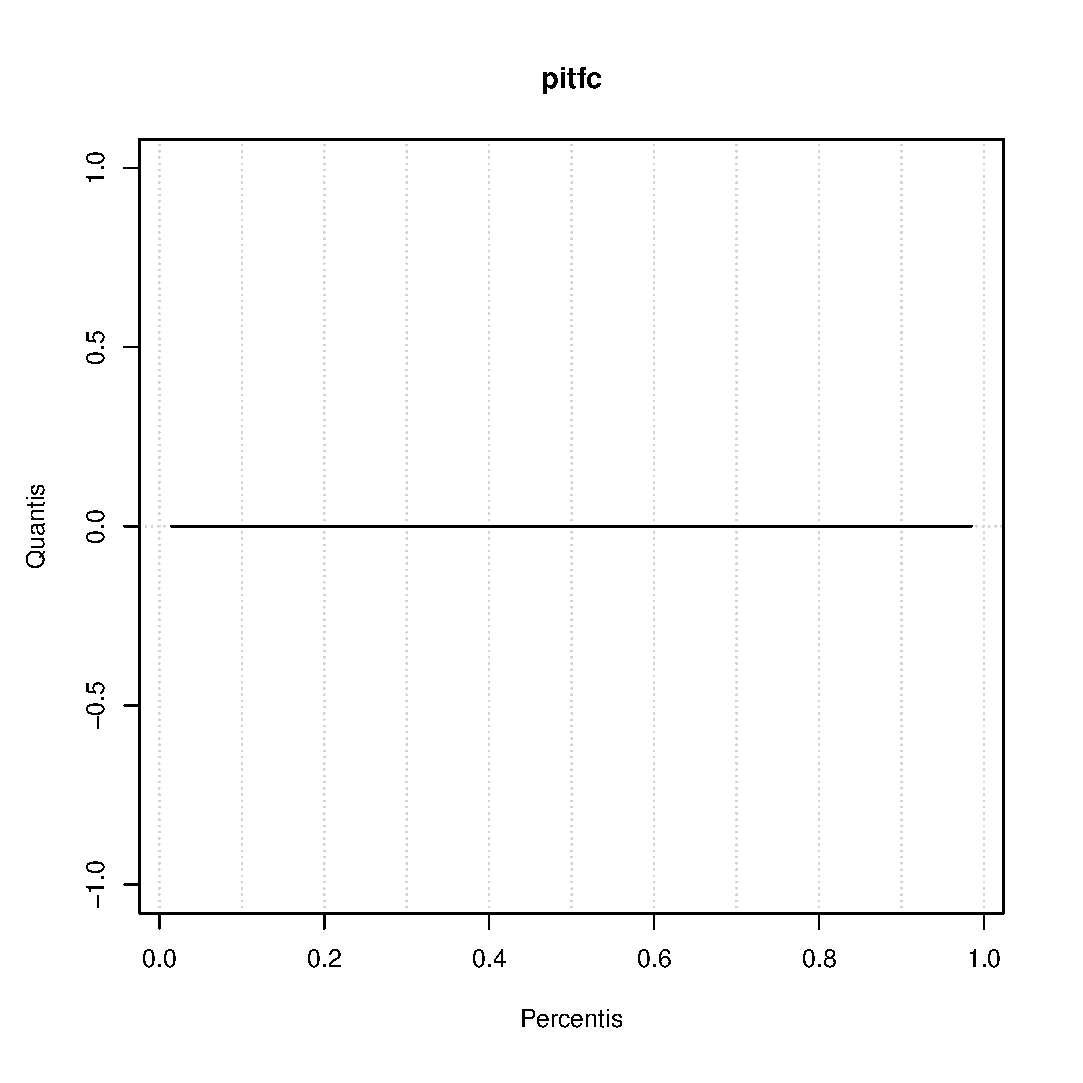
\includegraphics[width=0.6\textwidth]
      {dados/linux/pitfc.eps}
  \caption{Gráfico de Percentis da métrica PITFC}
\end{figure}

\begin{figure}[h]
  \centering
  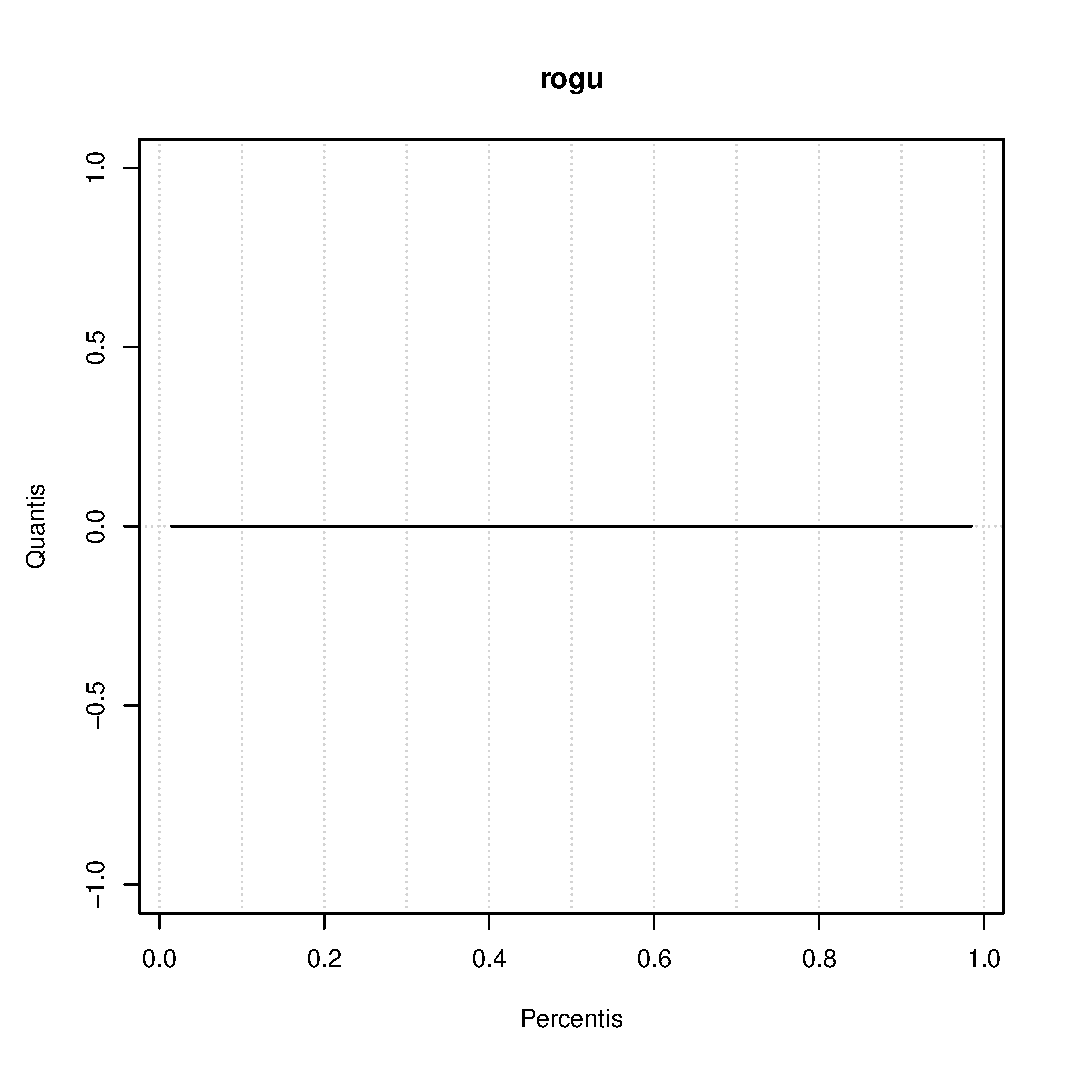
\includegraphics[width=0.6\textwidth]
      {dados/linux/rogu.eps}
  \caption{Gráfico de Percentis da métrica ROGU}
\end{figure}

\newpage

\begin{figure}[h]
  \centering
  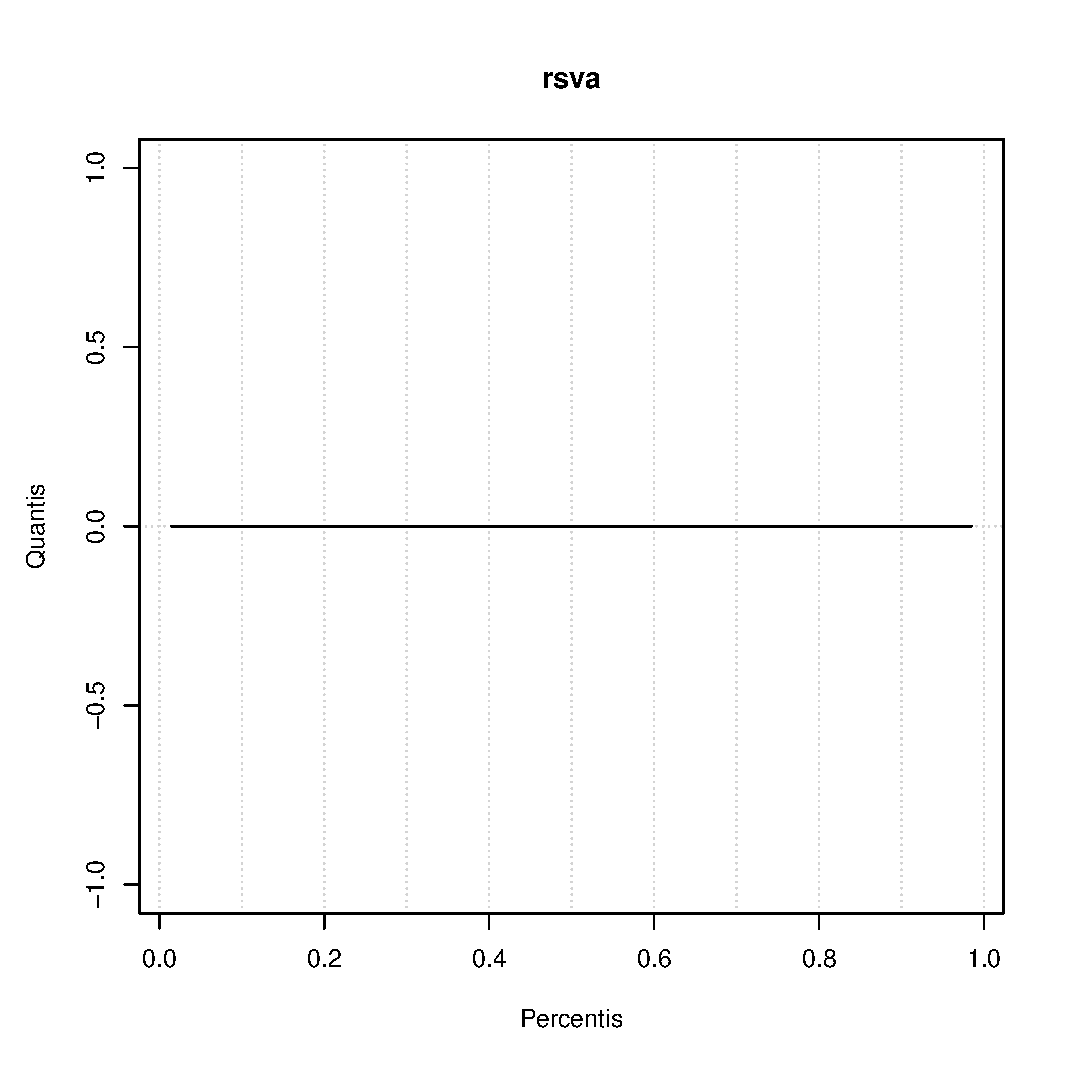
\includegraphics[width=0.6\textwidth]
      {dados/linux/rsva.eps}
  \caption{Gráfico de Percentis da métrica RSVA}
\end{figure}

\begin{figure}[h]
  \centering
  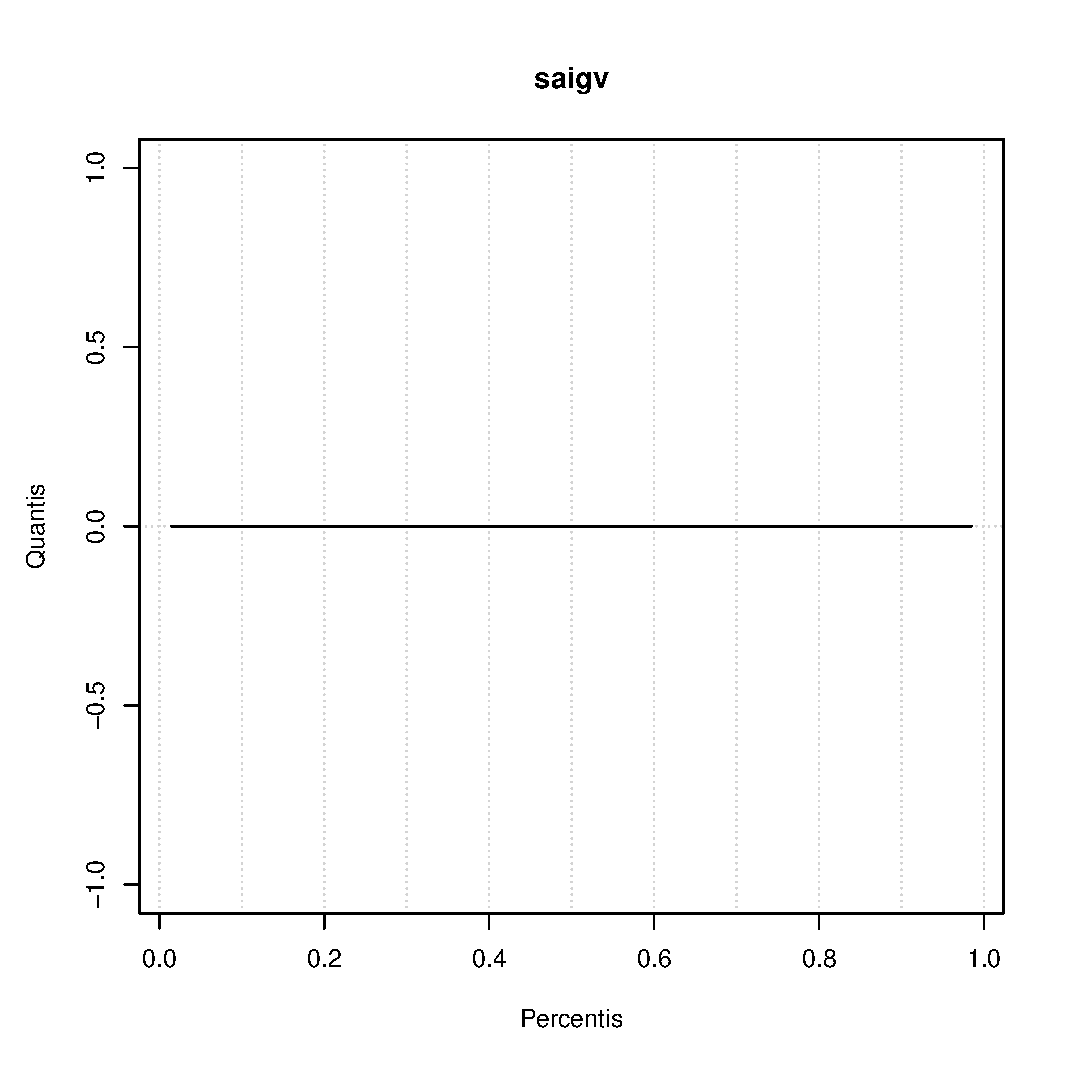
\includegraphics[width=0.6\textwidth]
      {dados/linux/saigv.eps}
  \caption{Gráfico de Percentis da métrica SAIGV}
\end{figure}

\newpage

\begin{figure}[h]
  \centering
  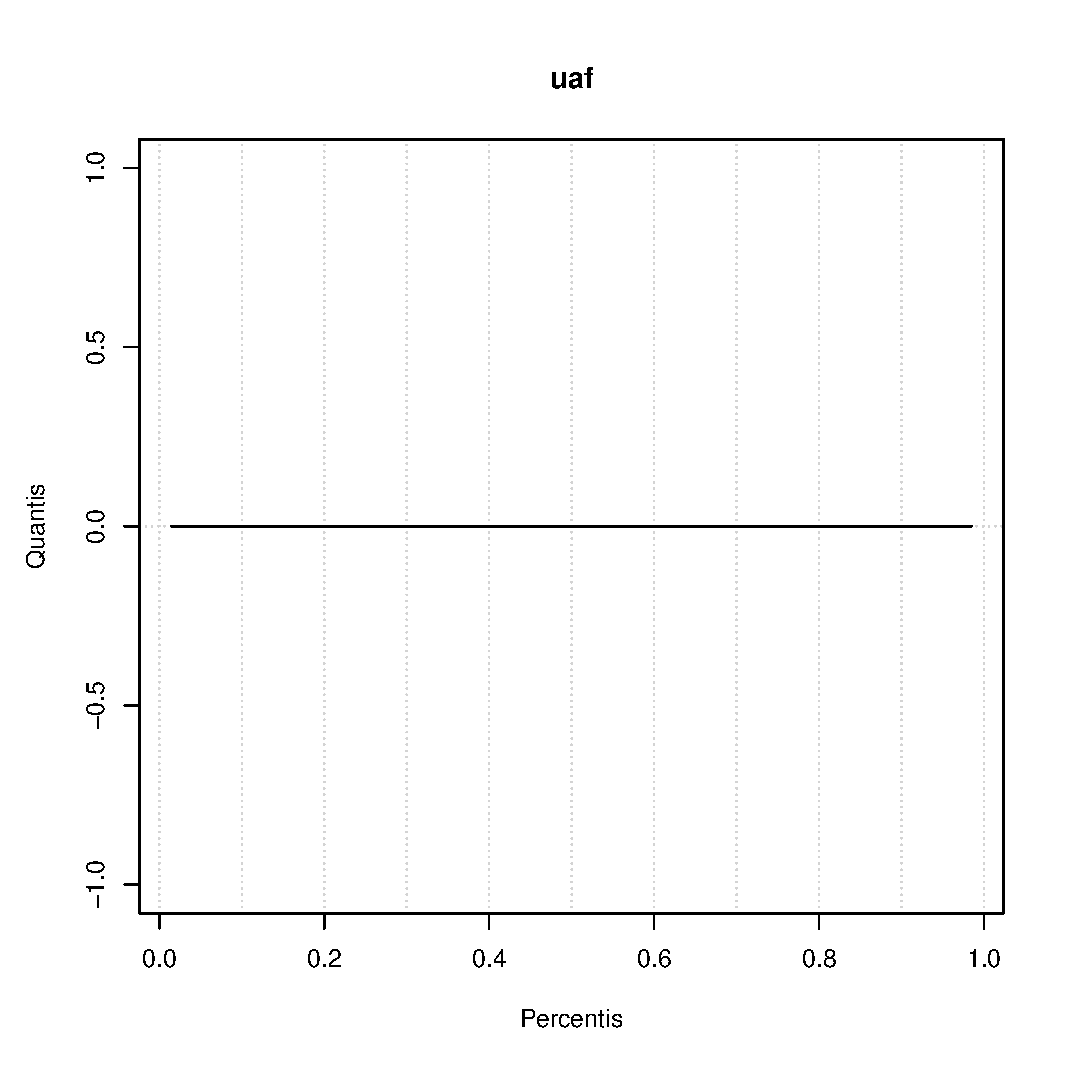
\includegraphics[width=0.6\textwidth]
      {dados/linux/uaf.eps}
  \caption{Gráfico de Percentis da métrica UAF}
\end{figure}

\begin{figure}[h]
  \centering
  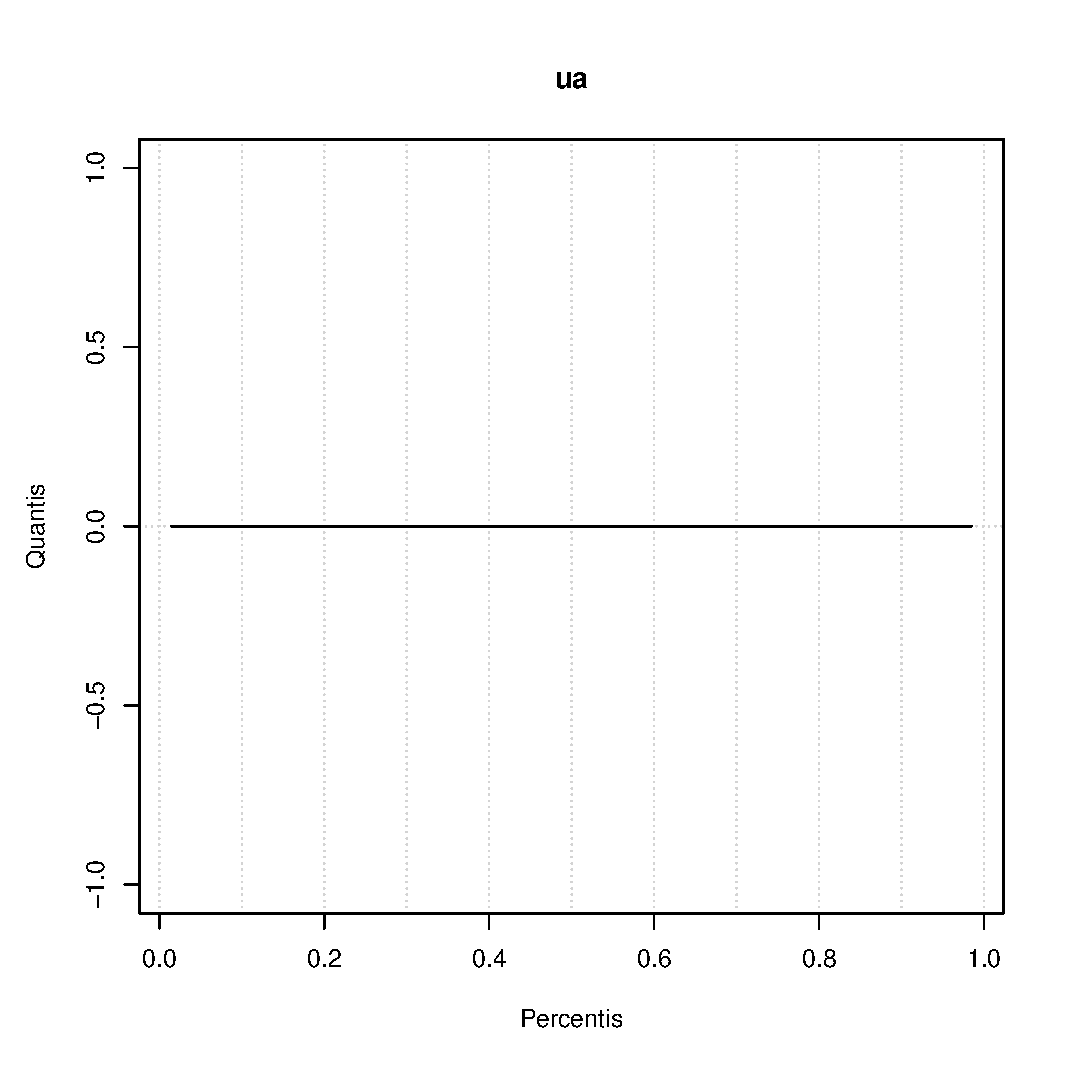
\includegraphics[width=0.6\textwidth]
      {dados/linux/ua.eps}
  \caption{Gráfico de Percentis da métrica UA}
\end{figure}

\newpage

\begin{figure}[h]
  \centering
  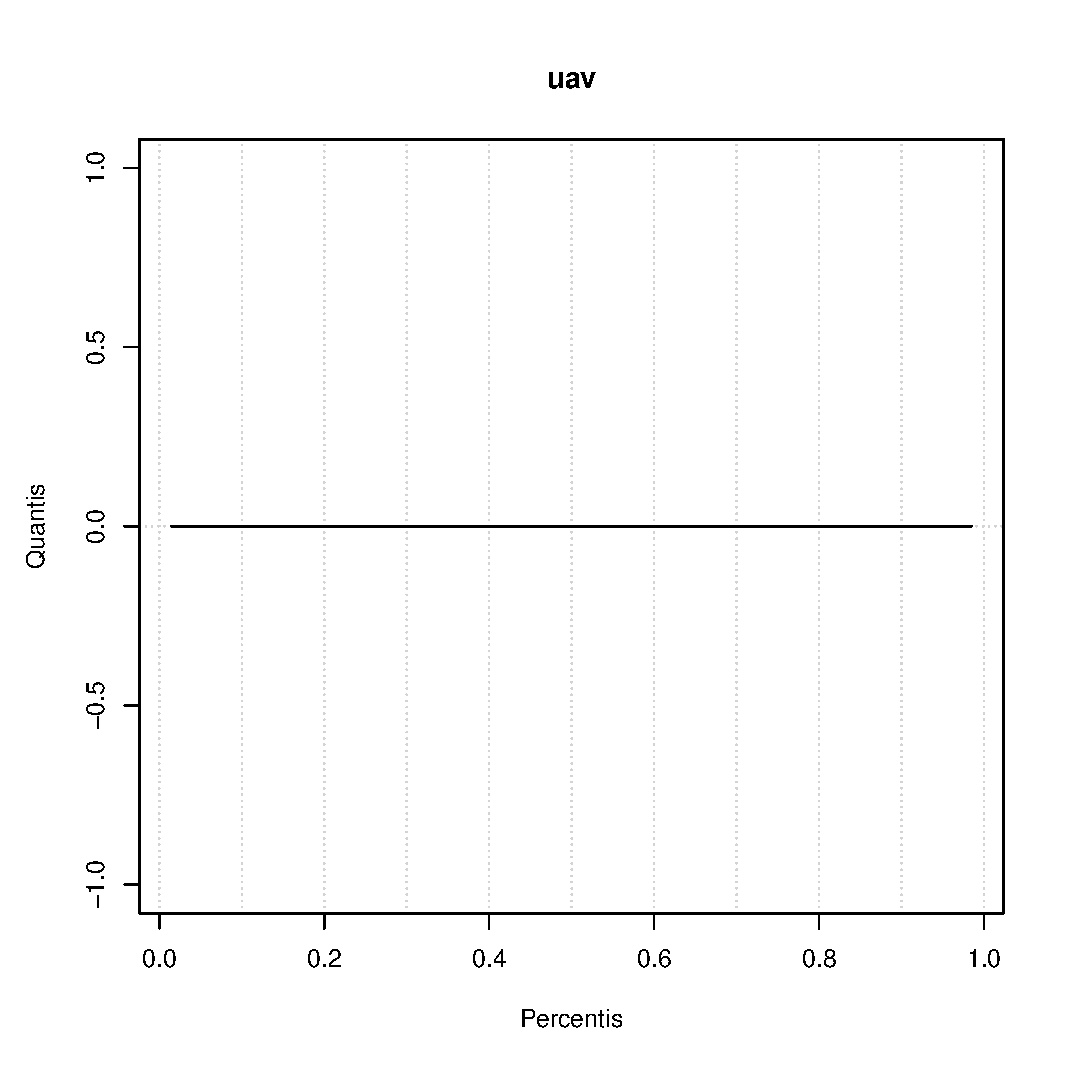
\includegraphics[width=0.6\textwidth]
      {dados/linux/uav.eps}
  \caption{Gráfico de Percentis da métrica UAV}
\end{figure}



\chapter{Análise Qualitativa} \label{anex:analise_qualitativa}

Neste anexo possui as tabelas de análise das métricas de vulnerabilidade de código fonte por módulo
dos projetos utilizados para realização da análise qualitativa, na seção \ref{sec:analise_qualitativa}.


\begin{table}[h]
\resizebox{\textwidth}{!}{%
\begin{tabular}{ccc}
\hline
\textbf{Métrica} & \textbf{Nº total de Módulos vulneráveis} & \textbf{\% de Módulos vulneráveis} \\ \hline
\rowcolor[HTML]{EFEFEF} 
\textbf{AN}      & 11                                       & 4.3478                             \\ \hline
\textbf{AUV}     & 2                                        & 0.7905                             \\ \hline
\rowcolor[HTML]{EFEFEF} 
\textbf{DNP}     & 22                                       & 8.6956                             \\ \hline
\textbf{MLK}     & 1                                        & 0.3952                             \\ \hline
\textbf{ROGU}    & 3                                        & 1.1857                             \\ \hline
\rowcolor[HTML]{EFEFEF} 
\textbf{UA}      & 1                                        & 0.3952                             \\ \hline
\textbf{UAV}     & 3                                        & 1.1857                             \\ \hline
\end{tabular}
}
\caption{Projeto Bash}
\end{table}



\begin{table}[h]
\resizebox{\textwidth}{!}{%
\begin{tabular}{ccc}
\hline
\textbf{Métrica} & \textbf{Nº total de Módulos vulneráveis} & \textbf{\% de Módulos vulneráveis} \\ \hline
\rowcolor[HTML]{EFEFEF} 
\textbf{AN}      & 7                                        & 0.4755                             \\ \hline
\textbf{AUV}     & 9                                        & 0.6114                             \\ \hline
\rowcolor[HTML]{EFEFEF} 
\textbf{DNP}     & 93                                       & 6.3179                             \\ \hline
\textbf{DUPV}    & 1                                        & 0.0679                             \\ \hline
\textbf{ROGU}    & 11                                       & 0.0563                             \\ \hline
\end{tabular}
}
\caption{Projeto Blender}
\end{table}





\begin{table}[h]
\resizebox{\textwidth}{!}{%
\begin{tabular}{ccc}
\hline
\textbf{Métrica} & \textbf{Nº total de Módulos vulneráveis} & \textbf{\% de Módulos vulneráveis} \\ \hline
\rowcolor[HTML]{EFEFEF} 
\textbf{AN}      & 10                                       & 0.5630                             \\ \hline
\textbf{AUV}     & 31                                       & 1.7454                             \\ \hline
\rowcolor[HTML]{EFEFEF} 
\textbf{DNP}     & 37                                       & 2.0833                             \\ \hline
\textbf{DUPV}    & 4                                        & 0.2252                             \\ \hline
\textbf{MLK}     & 1                                        & 0.0563                             \\ \hline
\rowcolor[HTML]{EFEFEF} 
\textbf{ROGU}    & 24                                       & 1.3513                             \\ \hline
\textbf{UAV}     & 13                                       & 1.1857                             \\ \hline
\end{tabular}
}
\caption{Projeto FFmpeg}
\end{table}




\begin{table}[h]
\resizebox{\textwidth}{!}{%
\begin{tabular}{ccc}
\hline
\textbf{Métrica} & \textbf{Nº total de Módulos vulneráveis} & \textbf{\% de Módulos vulneráveis} \\ \hline
\rowcolor[HTML]{EFEFEF} 
\textbf{AN}      & 29                                       & 0.2337                             \\ \hline
\textbf{ASOM}    & 7                                        & 0.0564                             \\ \hline
\rowcolor[HTML]{EFEFEF} 
\textbf{AUV}     & 24                                       & 0.1934                             \\ \hline
\textbf{DNP}     & 218                                      & 1.7574                             \\ \hline
\textbf{DUPV}    & 10                                       & 0.0806                             \\ \hline
\rowcolor[HTML]{EFEFEF} 
\textbf{MLK}     & 12                                       & 0.0967                             \\ \hline
\textbf{OBAA}    & 5                                        & 0.0403                             \\ \hline
\rowcolor[HTML]{EFEFEF} 
\textbf{ROGU}    & 34                                       & 0.2741                             \\ \hline
\textbf{SAIGV}   & 2                                        & 0.0161                             \\ \hline
\rowcolor[HTML]{EFEFEF} 
\textbf{UA}      & 6                                        & 0.0483                             \\ \hline
\textbf{UAF}     & 8                                        & 0.0644                             \\ \hline
\rowcolor[HTML]{EFEFEF} 
\textbf{UAV}     & 22                                       &                                    \\ \hline
\end{tabular}
}
\caption{Projeto Firefox}
\end{table}



\begin{table}[h]
\resizebox{\textwidth}{!}{%
\begin{tabular}{ccc}
\hline
\textbf{Métrica} & \textbf{Nº total de Módulos vulneráveis} & \textbf{\% de Módulos vulneráveis} \\ \hline
\rowcolor[HTML]{EFEFEF} 
\textbf{AN}      & 2                                        & 0.7575                             \\ \hline
\textbf{DNP}     & 16                                       & 6.0606                             \\ \hline
\rowcolor[HTML]{EFEFEF} 
\textbf{ROGU}    & 2                                        & 0.7575                             \\ \hline
\textbf{UAV}     & 4                                        & 1.5151                             \\ \hline
\end{tabular}
}
\caption{Projeto Gstreamer}
\end{table}




\begin{table}[h]
\resizebox{\textwidth}{!}{%
\begin{tabular}{ccc}
\hline
\textbf{Métrica} & \textbf{Nº total de Módulos vulneráveis} & \textbf{\% de Módulos vulneráveis} \\ \hline
\rowcolor[HTML]{EFEFEF} 
\textbf{AN}      & 3                                        & 0.1164                             \\ \hline
\textbf{AUV}     & 3                                        & 0.1164                             \\ \hline
\rowcolor[HTML]{EFEFEF} 
\textbf{DF}      & 1                                        & 0.0388                             \\ \hline
\textbf{DNP}     & 6                                        & 0.2329                             \\ \hline
\rowcolor[HTML]{EFEFEF} 
\textbf{MLK}     & 9                                        & 0.3493                             \\ \hline
\textbf{ROGU}    & 7                                        & 0.2717                             \\ \hline
\rowcolor[HTML]{EFEFEF} 
\textbf{SAIGV}   & 1                                        & 0.0388                             \\ \hline
\textbf{UA}      & 2                                        & 0.0776                             \\ \hline
\rowcolor[HTML]{EFEFEF} 
\textbf{UAF}     & 5                                        & 0.1940                             \\ \hline
\textbf{UAV}     & 3                                        & 3.2667                             \\ \hline
\end{tabular}
}
\caption{Projeto Inetutils}
\end{table}



\begin{table}[h]
\resizebox{\textwidth}{!}{%
\begin{tabular}{ccc}
\hline
\textbf{Métrica} & \textbf{Nº total de Módulos vulneráveis} & \textbf{\% de Módulos vulneráveis} \\ \hline
\rowcolor[HTML]{EFEFEF} 
\textbf{DNP}     & 40                                       & 0.1734                             \\ \hline
\textbf{DUPV}    & 3                                        & 0.0130                             \\ \hline
\rowcolor[HTML]{EFEFEF} 
\textbf{SAIGV}   & 1                                        & 0.0043                             \\ \hline
\end{tabular}
}
\caption{Projeto Linux Kernel}
\end{table}



\begin{table}[h]
\resizebox{\textwidth}{!}{%
\begin{tabular}{ccc}
\hline
\textbf{Métrica} & \textbf{Nº total de Módulos vulneráveis} & \textbf{\% de Módulos vulneráveis} \\ \hline
\rowcolor[HTML]{EFEFEF} 
\textbf{AN}      & 2                                        & 0.8064                             \\ \hline
\textbf{DNP}     & 7                                        & 2.8225                             \\ \hline
\rowcolor[HTML]{EFEFEF} 
\textbf{MLK}     & 2                                        & 0.8064                             \\ \hline
\textbf{UA}      & 1                                        & 0.4032                             \\ \hline
\textbf{UAF}     & 4                                        & 0.1026                             \\ \hline
\end{tabular}
}
\caption{Projeto OpenSSH}
\end{table}





\begin{table}[h]
\resizebox{\textwidth}{!}{%
\begin{tabular}{ccc}
\hline
\textbf{Métrica} & \textbf{Nº total de Módulos vulneráveis} & \textbf{\% de Módulos vulneráveis} \\ \hline
\rowcolor[HTML]{EFEFEF} 
\textbf{AN}      & 6                                        & 0.6160                             \\ \hline
\textbf{AUV}     & 1                                        & 0.1026                             \\ \hline
\rowcolor[HTML]{EFEFEF} 
\textbf{DNP}     & 14                                       & 1.4373                             \\ \hline
\textbf{ROGU}    & 6                                        & 0.6160                             \\ \hline
\textbf{UAV}     & 1                                        & 0.7472                             \\ \hline
\end{tabular}
}
\caption{Projeto OpenSSL}
\end{table}





\begin{table}[h]
\resizebox{\textwidth}{!}{%
\begin{tabular}{ccc}
\hline
\textbf{Métrica} & \textbf{Nº total de Módulos vulneráveis} & \textbf{\% de Módulos vulneráveis} \\ \hline
\rowcolor[HTML]{EFEFEF} 
\textbf{AN}      & 2                                        & 0.3629                             \\ \hline
\textbf{AUV}     & 4                                        & 0.7259                             \\ \hline
\rowcolor[HTML]{EFEFEF} 
\textbf{BF}      & 1                                        & 0.1814                             \\ \hline
\textbf{DNP}     & 18                                       & 3.2667                             \\ \hline
\rowcolor[HTML]{EFEFEF} 
\textbf{DUPV}    & 2                                        & 0.3629                             \\ \hline
\textbf{MLK}     & 2                                        & 0.3629                             \\ \hline
\rowcolor[HTML]{EFEFEF} 
\textbf{OBAA}    & 2                                        & 0.3629                             \\ \hline
\textbf{ROGU}    & 6                                        & 1.0889                             \\ \hline
\rowcolor[HTML]{EFEFEF} 
\textbf{UA}      & 1                                        & 0.1814                             \\ \hline
\textbf{UAV}     & 1                                        & 0.1164                             \\ \hline
\end{tabular}
}
\caption{Projeto Python2.7}
\end{table}




\begin{table}[h]
\resizebox{\textwidth}{!}{%
\begin{tabular}{ccc}
\hline
\textbf{Métrica} & \textbf{Nº total de Módulos vulneráveis} & \textbf{\% de Módulos vulneráveis} \\ \hline
\rowcolor[HTML]{EFEFEF} 
\textbf{AN}      & 4                                        & 1.0498                             \\ \hline
\textbf{ASOM}    & 2                                        & 0.5249                             \\ \hline
\rowcolor[HTML]{EFEFEF} 
\textbf{AUV}     & 2                                        & 0.5249                             \\ \hline
\textbf{DNP}     & 10                                       & 2.6246                             \\ \hline
\textbf{MLK}     & 1                                        & 0.2624                             \\ \hline
\rowcolor[HTML]{EFEFEF} 
\textbf{ROGU}    & 2                                        & 0.5249                             \\ \hline
\textbf{SAIGV}   & 1                                        & 0.2624                             \\ \hline
\rowcolor[HTML]{EFEFEF} 
\textbf{UAF}     & 1                                        & 0.2624                             \\ \hline
\textbf{UAV}     & 1                                        & 0.1814                             \\ \hline
\end{tabular}
}
\caption{Projeto Ruby-2.1}
\end{table}


\end{apendicesenv}
